\documentclass[a5paper, 10pt]{article}

% Текст
\usepackage[utf8]{inputenc} % UTF-8 кодировка
\usepackage[russian]{babel} % Русский язык
\usepackage{indentfirst} % красная строка в первом параграфе в главе
% Отображение страниц
\usepackage{geometry} % размеры листа и отступов
\geometry{
	left=12mm,
	top=25mm,
	right=15mm,
	bottom=17mm,
	marginparsep=0mm,
	marginparwidth=0mm,
	headheight=10mm,
	headsep=7mm,
	nofoot}
 
\usepackage{afterpage,fancyhdr} % настройка колонтитулов
\pagestyle{fancy}
\fancypagestyle{style}{ % создание нового стиля style
	\fancyhf{} % очистка колонтитулов
	\fancyhead[LO, RE]{Слежение и компенсация} % название документа наверху
	\fancyhead[RO, LE]{\leftmark} % название section наверху
	\fancyfoot[RO, LE]{\thepage} % номер страницы справа внизу на нечетных и слева внизу на четных
	\renewcommand{\headrulewidth}{0.25pt} % толщина линии сверху
	\renewcommand{\footrulewidth}{0pt} % толцина линии снизу
}
\fancypagestyle{plain}{ % создание нового стиля plain -- полностью пустого
	\fancyhf{}
	\renewcommand{\headrulewidth}{0pt}
}
\fancypagestyle{title}{ % создание нового стиля title -- для титульной страницы
	\fancyhf{}
	\fancyhead[C]{{\footnotesize
			Министерство образования и науки Российской Федерации\\
			Федеральное государственное автономное образовательное учреждение высшего образования
	}}
	\fancyfoot[C]{{\large 
			Санкт-Петербург, 2023-2024
	}}
	\renewcommand{\headrulewidth}{0pt}
}

% Математика
\usepackage{amsmath, amsfonts, amssymb, amsthm} % Набор пакетов для математических текстов
\usepackage{dmvnbase} % мехматовский пакет latex-сокращений
\usepackage{cancel} % зачеркивание для сокращений
% Рисунки и фигуры
\usepackage[pdftex]{graphicx} % вставка рисунков
\usepackage{wrapfig, subcaption} % вставка фигур, обтекая текст
\usepackage{caption} % для настройки подписей
\captionsetup{figurewithin=none,labelsep=period, font={small,it}} % настройка подписей к рисункам
% Рисование
\usepackage{tikz} % рисование
\usepackage{pgfplots} % графики
% Таблицы
\usepackage{multirow} % объединение строк
\usepackage{multicol} % объединение столбцов
% Остальное
\usepackage[unicode, pdftex]{hyperref} % гиперссылки
\usepackage{enumitem} % нормальное оформление списков
\setlist{itemsep=0.15cm,topsep=0.15cm,parsep=1pt} % настройки списков
% Теоремы, леммы, определения...
\theoremstyle{definition}
\newtheorem{Def}{Определение}
\newtheorem*{Axiom}{Аксиома}
\theoremstyle{plain}
\newtheorem{Th}{Теорема}
\newtheorem{Lem}{Лемма}
\newtheorem{Cor}{Следствие}
\newtheorem{Ex}{Пример}
\theoremstyle{remark}
\newtheorem*{Note}{Замечание}
\newtheorem*{Solution}{Решение}
\newtheorem*{Proof}{Доказательство}
% Свои команды
\newcommand{\comb}[1]{\left[\hspace{-4pt}\begin{array}{l}#1\end{array}\right.\hspace{-5pt} } % совокупность уравнений
\usepackage{listings}
\usepackage{color}
% Титульный лист
\newcommand*{\titlePage}{
	\thispagestyle{title}
	\begingroup
	\begin{center}
%		{\footnotesize
%			Министерство образования и науки Российской Федерации\\
%			Федеральное государственное автономное образовательное учреждение высшего образования
%		}
%		
		\vspace*{6ex}
		
		{\small
			САНКТ-ПЕТЕРБУРГСКИЙ НАЦИОНАЛЬНЫЙ ИССЛЕДОВАТЕЛЬСКИЙ УНИВЕРСИТЕТ ИНФОРМАЦИОННЫХ ТЕХНОЛОГИЙ, МЕХАНИКИ И ОПТИКИ	
		}
		
		\vspace*{2ex}
		
		{\normalsize
			Факультет систем управления и робототехники
		}
		
		\vspace*{15ex}
		
		{\Large \bfseries 
			Отчет по лабораторной работе №1 \\ 
			по дисциплине "Адаптивное и робастное управление"\\
   
            Вариант 4
		}
	\end{center}
	\vspace*{20ex}
	\begin{flushright}
		{\large 
			\underline{Выполнил}: студенты гр. \textbf{R34353}\\
			\begin{flushright}
				\textbf{Симонов Р. А.}\\
                    \textbf{Золотарев Д. В.}\\
			\end{flushright}
		}
		
		\vspace*{5ex}
		
		{\large 
			\underline{Преподаватель}: \textit{Герасимов Д. Н.}
		}
	\end{flushright}	
	\newpage
	\setcounter{page}{1}
	\endgroup}
	

\begin{document}
	\titlePage
	\pagestyle{style}

    \tableofcontents
    \newpage
    
    \section{Цель работы}
        Построить неадаптивные и адаптивные системы управления, провести моедлирование полученных систем, сравнить качество переходного процесса
        
    \section{Ход работы}
        \subsection{Постановка задачи}
            Рассмотрим объект 

$$
    \dot{x} = \theta x + u
$$

где $x$ - выход объекта (совпадает с переменной состояния), $u$ - сигнал
управления, $\theta$ - неизвестный постоянный параметр. Хотим компенсировать неопределенности $\theta$ и обеспечить выполнение следующего целевого равенства:

\begin{equation}
    \lim_{t \rightarrow \infty} (x_m(t) - x(t)) = \lim_{t \rightarrow \infty} \varepsilon(t) = 0
    \label{goal}
\end{equation}

где $\varepsilon = x_m - x$ - ошибка управления, $x_m$ - эталонный сигнал, являющийся выходом динамической модели (эталонной модели):

$$
    \dot{x}_m = -\lambda x_m + \lambda g
$$

где $g$ - кусочно-непрерывный ограниченный сигнал задания, $\lambda > 0$ параметр, задающий время переходного процесса.
        \subsection{Построение неадаптивной системы управления}
            Предположим, что параметр $\theta$ известен, тогда управление может быть легко найдено, как:

\begin{equation}
    u = -\theta x - \lambda x + \lambda g
    \label{control}
\end{equation}

Проведем моделирование полученной замкнутой системы в условиях скачкообразного трехкратного увеличения параметра $\theta$, получим следующие графики:

\begin{figure}
    \centerline{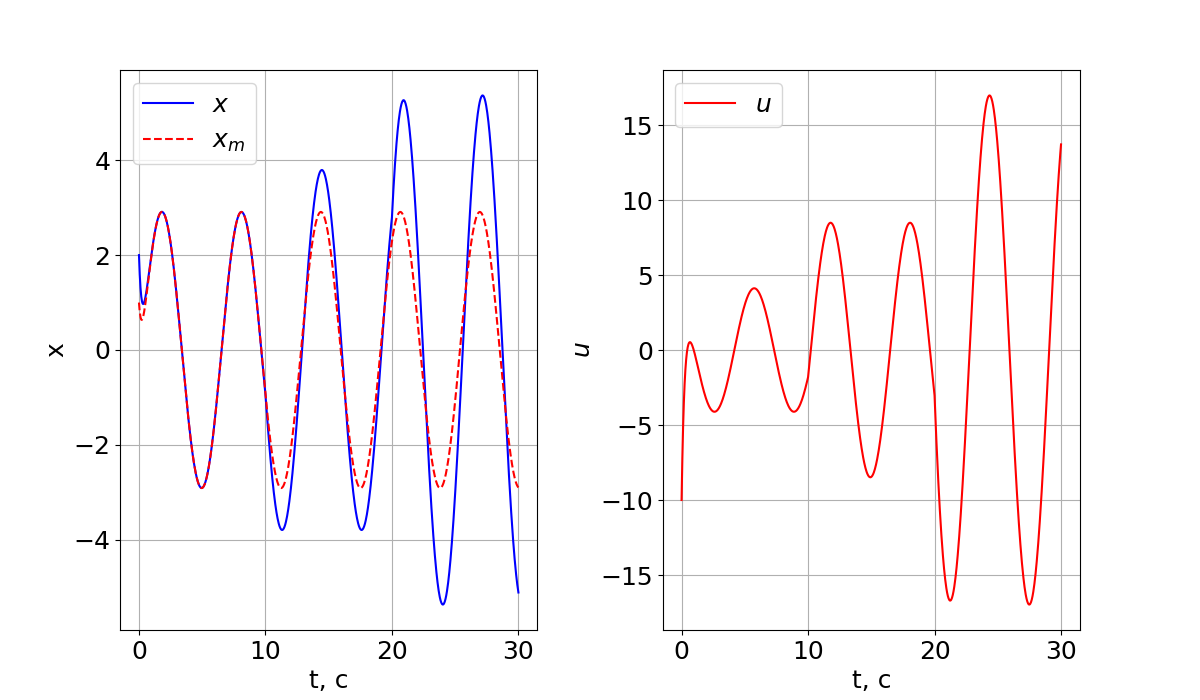
\includegraphics[width=\linewidth]{images/task_1.png}}
    \caption{График переходного процесса и управляющего воздействия для неадаптивной системы}
    \label{10}
\end{figure}

Как можно видеть, замкнутая система идеально следит за сигналом.
Попробуем теперь промоделировать таким образом, чтобы регулятор не знал об изменении параметра $\theta$ (то есть регулятор считает, что $\theta$ - известная константа)

\begin{figure}
    \centerline{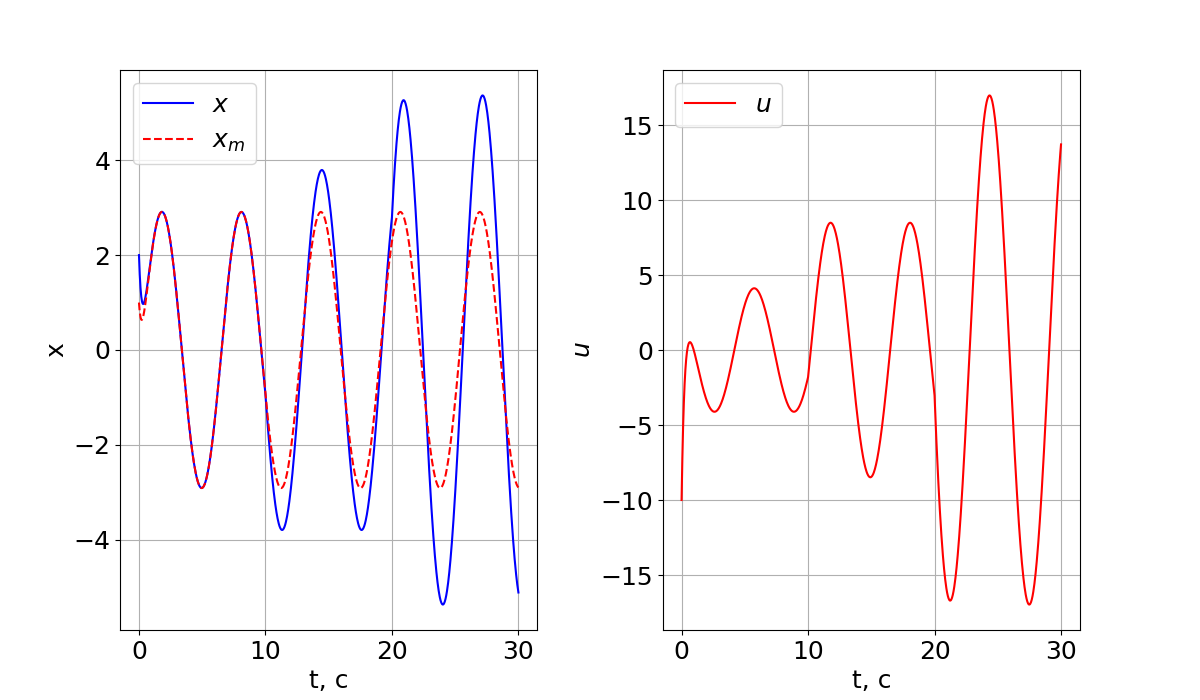
\includegraphics[width=\linewidth]{images/task_1_2.png}}
    \caption{График переходного процесса и управляющего воздействия для неадаптивной системы, при константном параметре $\theta$ при расчете управления}
    \label{11}
\end{figure}

До изменения параметра $\theta$ система идеально следила за эталонным сигналом, но после изменения, логичным образом, наблюдаем как система совершенно не справляется с задачей.


        \subsection{Построение адаптивной системы управления}
            Пусть теперь, как в исходной постановке задачи, параметр $\theta$ неизвестен. Тогда для реализуемости закона управления (\ref{control}) заменим величину $\theta$ на ее оценку $\hat{\theta}$:

\begin{equation}
    u = - \hat{\theta} x - \lambda x + \lambda g
\end{equation}

Если оценка $\hat{\theta}$ такая что, $\dot{\hat{\theta}} = - \gamma x \varepsilon$, где $\gamma$ - коэффициентом адаптации, то по методу функций Ляпунова можно показать, что целевое равенство (\ref{goal}) будет выполнено.

Проведем моделирование полученной замкнутой системы при различных значениях параметра $\gamma$, получим следующие графики:

\begin{figure}
    \centerline{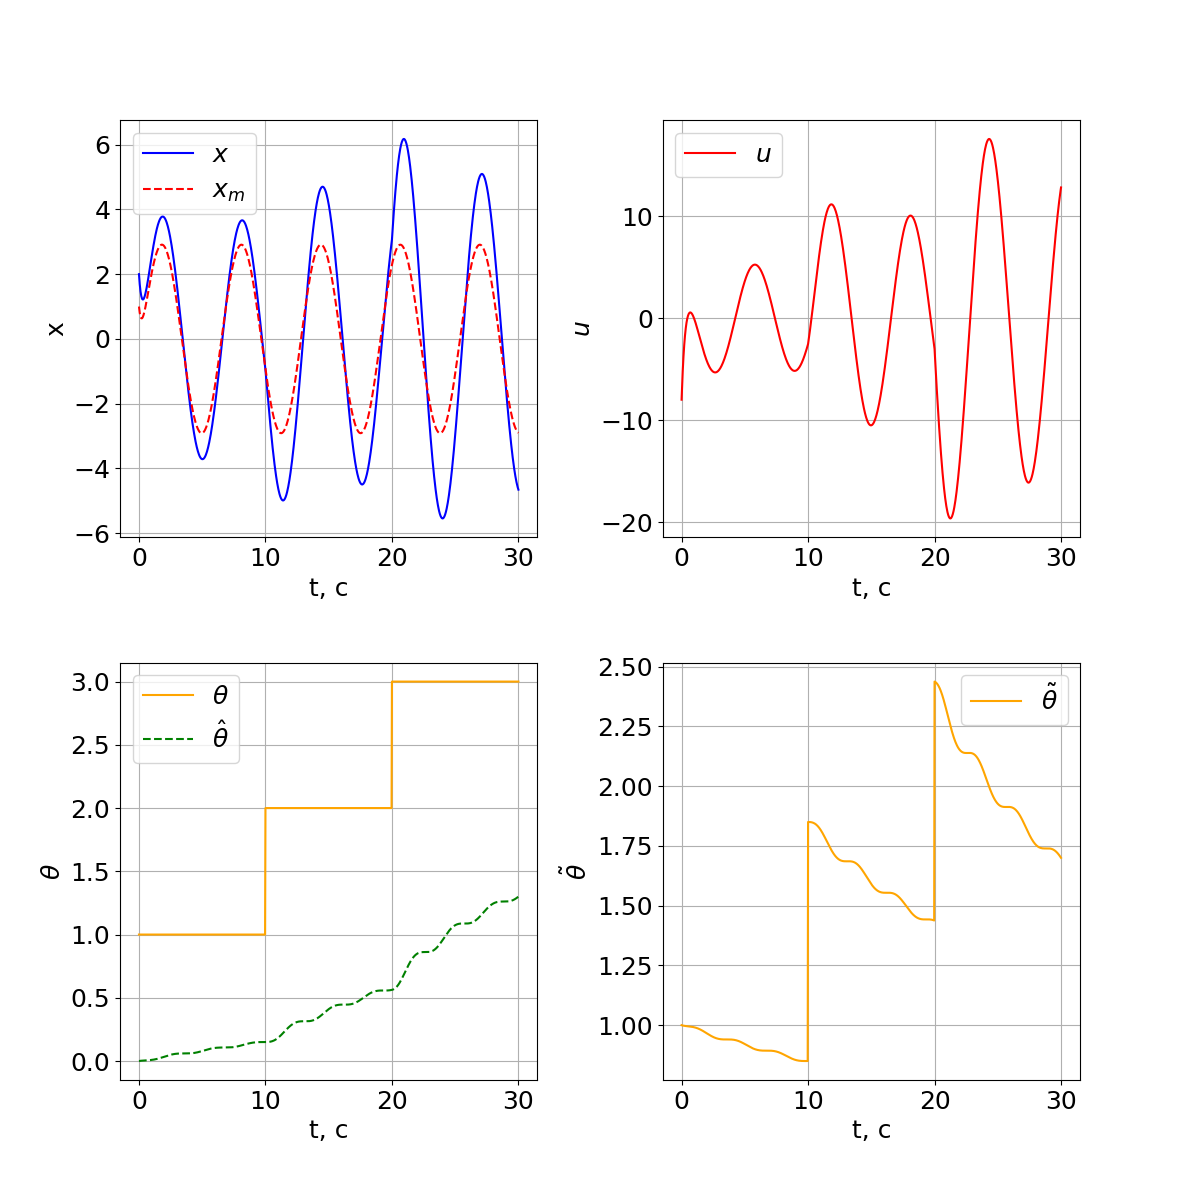
\includegraphics[width=\linewidth]{images/task_2_0.01.png}}
    \caption{График переходного процесса и управляющего воздействия, а также графика параметра $\theta$ и его оценки $\hat{\theta}$ для адаптивной системы с параметром $\gamma = 0.01$}
    \label{21}
\end{figure}

Как можно видеть, при маленьком коэффициенте адаптации, система не успевает дать правильную оценку параметру, так как изменение реального параметра происходит быстрее. Но при этом, целевое равенство (\ref{goal}) выполняется.

Рассмотрим результаты моделирования при других параметров $\gamma$:

\begin{figure}
    \centerline{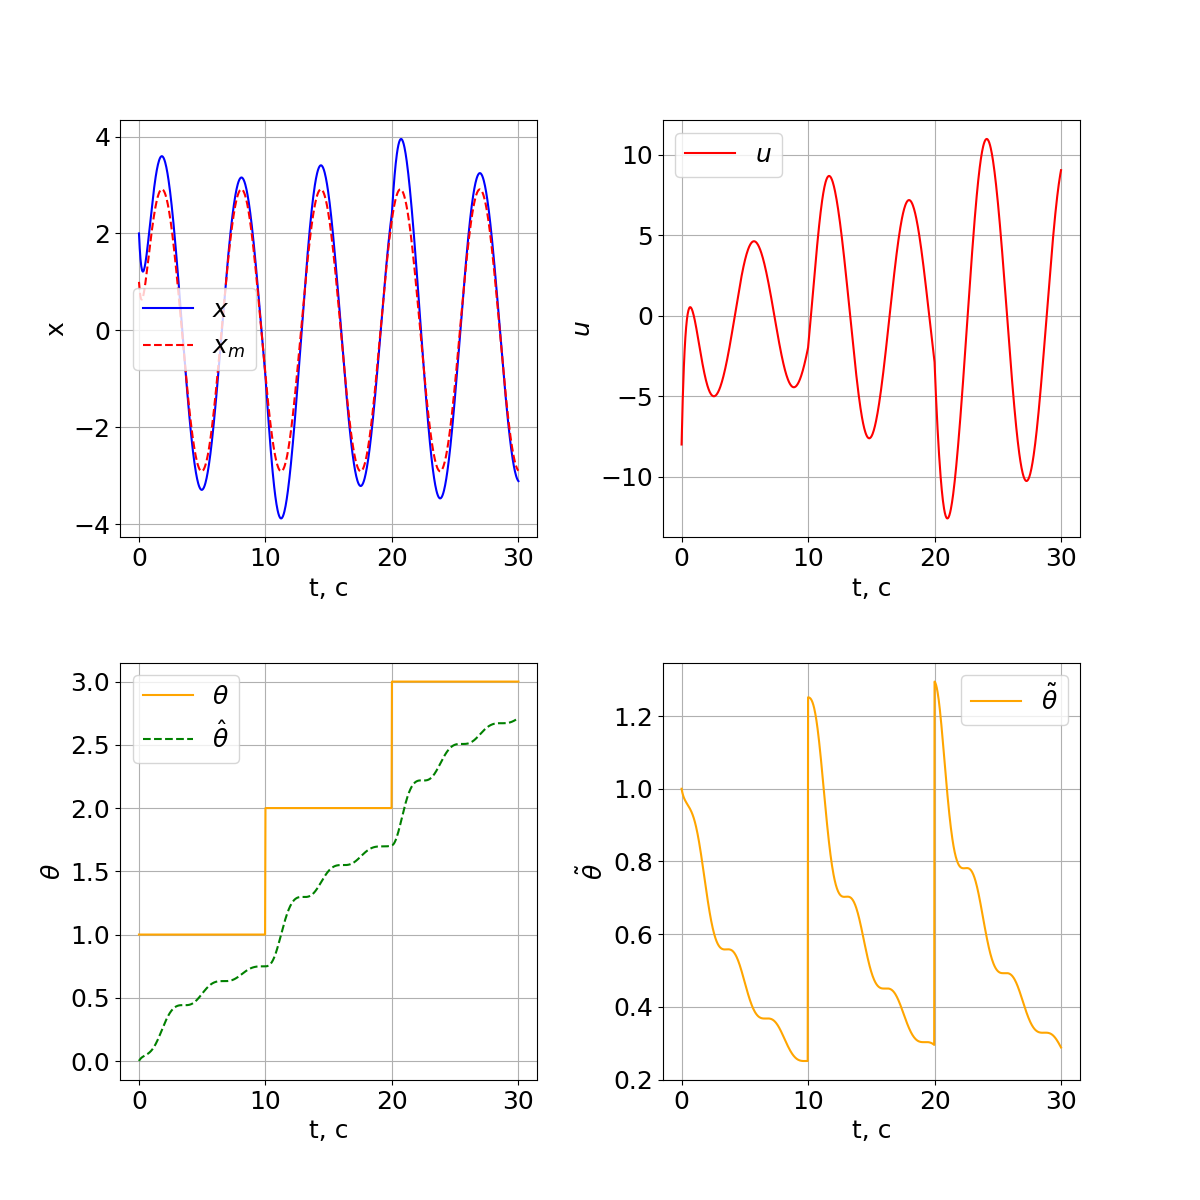
\includegraphics[width=\linewidth]{images/task_2_0.1.png}}
    \caption{График переходного процесса и управляющего воздействия, а также графика параметра $\theta$ и его оценки $\hat{\theta}$ для адаптивной системы с параметром $\gamma = 0.1$}
    \label{22}
\end{figure}

\begin{figure}
    \centerline{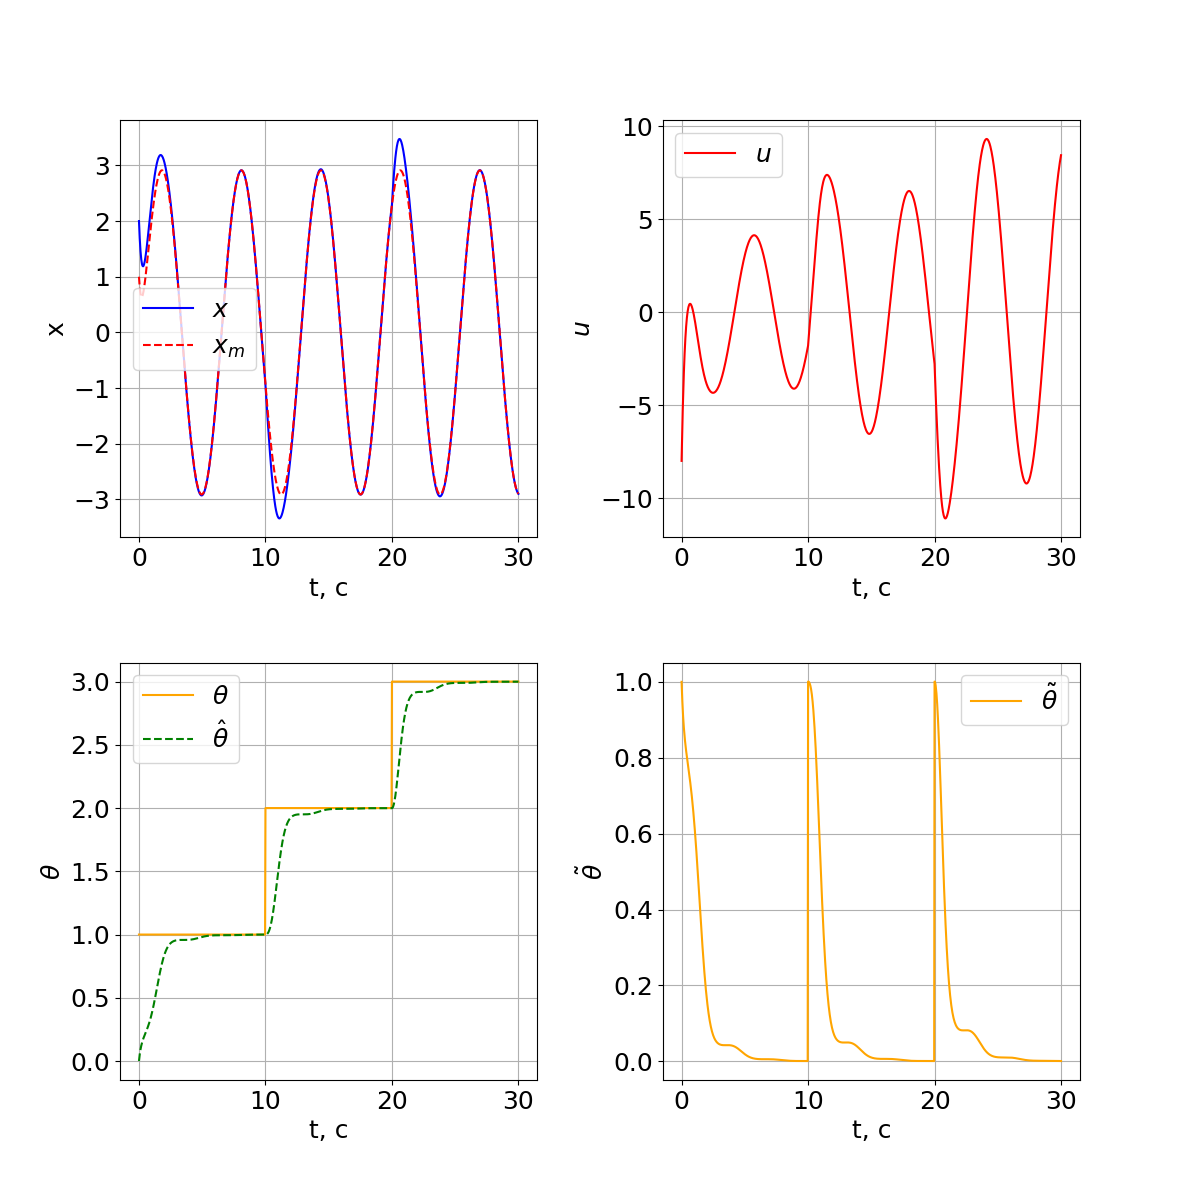
\includegraphics[width=\linewidth]{images/task_2_0.5.png}}
    \caption{График переходного процесса и управляющего воздействия, а также графика параметра $\theta$ и его оценки $\hat{\theta}$ для адаптивной системы с параметром $\gamma = 0.5$}
    \label{23}
\end{figure}

\begin{figure}
    \centerline{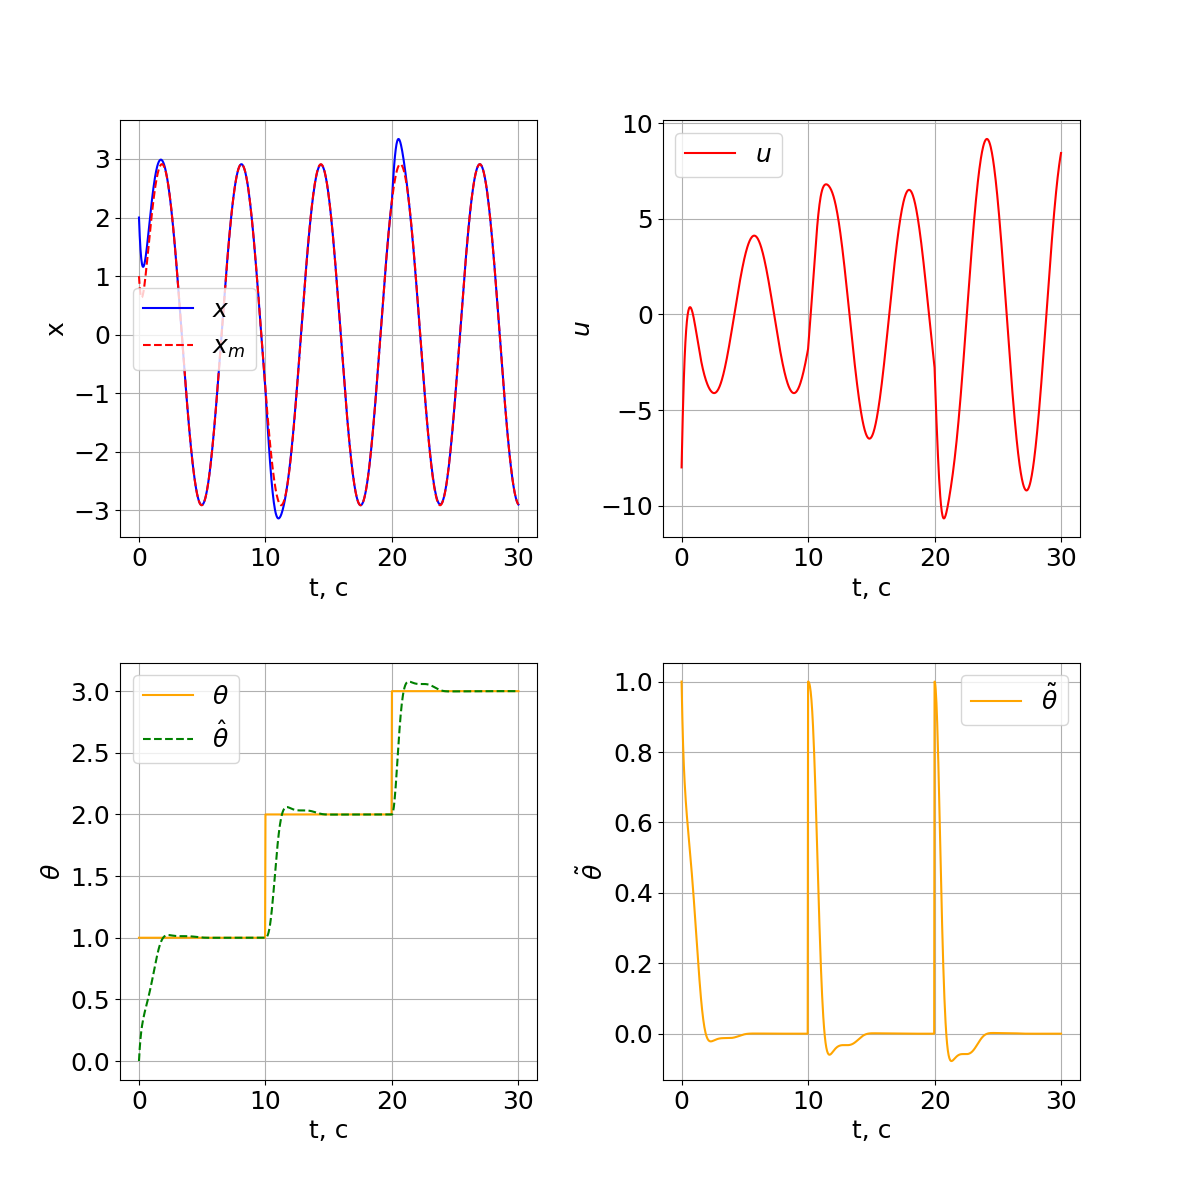
\includegraphics[width=\linewidth]{images/task_2_1.0.png}}
    \caption{График переходного процесса и управляющего воздействия, а также графика параметра $\theta$ и его оценки $\hat{\theta}$ для адаптивной системы с параметром $\gamma = 1.0$}
    \label{24}
\end{figure}

\begin{figure}
    \centerline{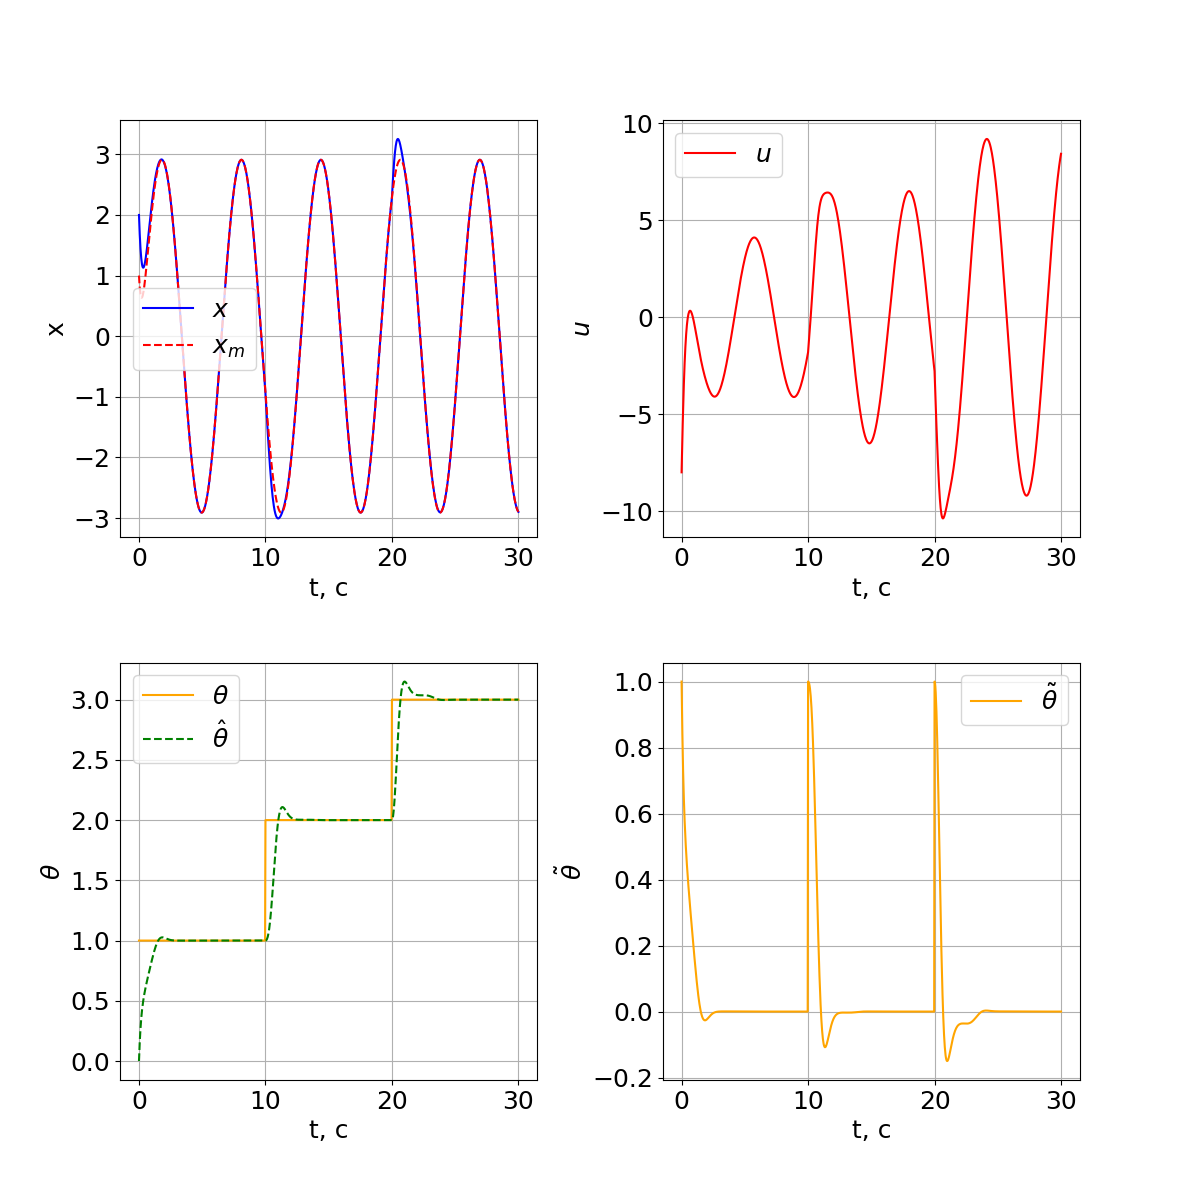
\includegraphics[width=\linewidth]{images/task_2_1.5.png}}
    \caption{График переходного процесса и управляющего воздействия, а также графика параметра $\theta$ и его оценки $\hat{\theta}$ для адаптивной системы с параметром $\gamma = 1.5$}
    \label{25}
\end{figure}

Можно заметить, что чем больше параметр $\gamma$, тем быстрее алгоритм адаптации сводит ошибку $\tilde{\theta}$ к нулю, и значит тем быстрее система адаптируются к скачкообразным изменениям параметра $\theta$.
        \subsection{Выводы}  
            В результате проделанной работы, были синтезированы неадаптивные и адаптивные системы управления. При известных параметрах, недапативный алгоритм идеально справляется с задачей, однако, такая ситуация в реально жизни встречается крайне редко. Кроме того, если недаптивный алгоритм будет знать только первоначальное значение параметров, то при малейшем его изменинии целевая задача не будет выполняться. 

            С другой стороны, адаптивный регулятор показывает хорошие результаты сходимости выхода объекта к выходу эталонной модели, несмотря на отсутствие информации о реальных значениях параметров объекта. Также было установлено, что чем больше коэффициент адаптации, тем быстрее ошибка между реальными значениями параметров и их оценками сводится к нулю.
            
\end{document}